\documentclass[border=10pt]{standalone}
\usepackage{pgfplots}
\usepgfplotslibrary{groupplots}
\pgfplotsset{compat=1.18}
\begin{document}
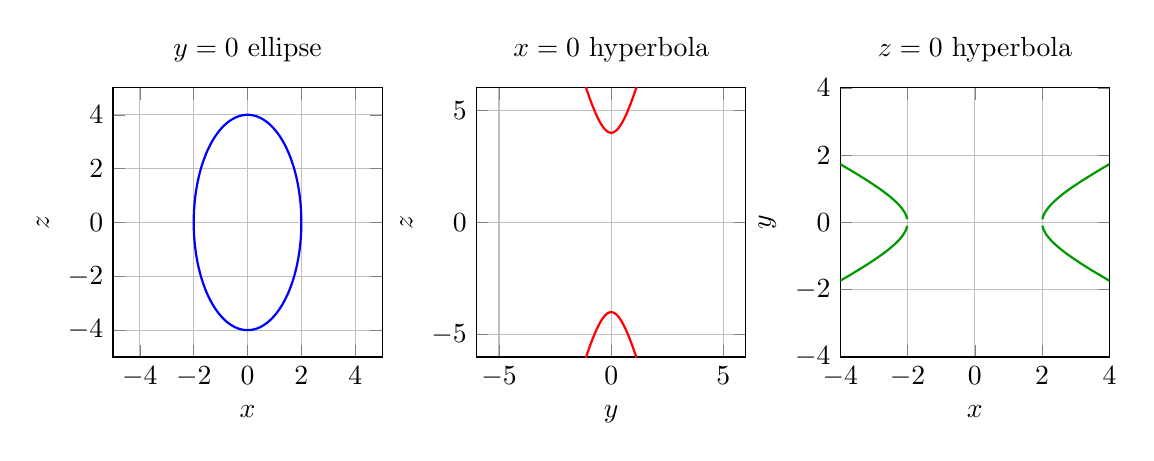
\begin{tikzpicture}
\begin{groupplot}[
    group style={group size=3 by 1, horizontal sep=1.2cm},
    axis equal,
    grid=both,
    width=5cm,
    height=5cm
]
\nextgroupplot[title={$y=0$ ellipse}, xlabel=$x$, ylabel=$z$, xmin=-3, xmax=3, ymin=-5, ymax=5]
\addplot[blue,thick,domain=0:360,samples=200] ({2*cos(x)},{4*sin(x)});

\nextgroupplot[title={$x=0$ hyperbola}, xlabel=$y$, ylabel=$z$, xmin=-3, xmax=3, ymin=-6, ymax=6]
\addplot[red,thick,domain=-3:3,samples=200] {4*sqrt(1+x^2)};
\addplot[red,thick,domain=-3:3,samples=200] {-4*sqrt(1+x^2)};

\nextgroupplot[title={$z=0$ hyperbola}, xlabel=$x$, ylabel=$y$, xmin=-4, xmax=4, ymin=-3, ymax=3]
\addplot[green!60!black,thick,domain=-4:-1,samples=200] {sqrt(x^2/4-1)};
\addplot[green!60!black,thick,domain=-4:-1,samples=200] {-sqrt(x^2/4-1)};
\addplot[green!60!black,thick,domain=1:4,samples=200] {sqrt(x^2/4-1)};
\addplot[green!60!black,thick,domain=1:4,samples=200] {-sqrt(x^2/4-1)};
\end{groupplot}
\end{tikzpicture}
\end{document}
